%----------------------------------------------------------------------------
\chapter{Rendszer specifikációja}
%----------------------------------------------------------------------------

\section {Felhasználói követelmények}

Egyetlen felhasználói típusunk van az applikációban: a tanuló, amely nyelvi készségeit fejleszteni kívánja.

\begin{itemize}
    \item \textbf{Platform}
    
    Egy mobilalkalmazás formájában a tanulni vágyó felhasználók mesterséges intelligencia segítségével gyakorolhatják a célnyelvet, ahol fejlődésüket tudják követni, különböző gyakorló feladatokat végezni és a beszédkészségükön dolgozni.

    \item \textbf{Regisztráció oldal}

    A felhasználó a szükséges adatok megadásával fiókot hozhat létre a platformon. Ennek elvégzése után kaphat hozzáférést az alkalmazás lényegi funkcióihoz.

    \item \textbf{Bejelentkezés oldal}

    A már létrehozott fiókba bejelentkezhet a felhasználó az email cím és jelszó megadásával. Sikeres bejelentkezés után pedig máris nekiláthat a nyelvtanulásnak.

    \item \textbf{Onboarding oldal}

    Az első bejelentkezés után a felhasználó kiválaszthatja a tanulni kívánt nyelvet, tanulási célját és egy kis felmérés után személyre szabott rendszert használhatja.

    \item \textbf{Főoldal}

    A főoldalon a felhasználó több gombbal is találkozik, amelyek különböző oldalakra vezetnek. Itt megtekintheti a legutóbbi beszélgetéseket, napi ajánlásokat, hiba összegzéseket, illetve egy gomb segítségével azonnal beszélgetést indíthat a mesterséges intelligenciával. Ugyanitt láthatja a profil oldalát is illetve a gyakorlást indító gombot is. Az oldal célja, hogy egy egységes helyen megtalálhassa a fő funkciókat a felhasználó.

    \item \textbf{Napi ajánlás oldal}

    Személyre szabott ajánlásokkal találkozhatnak ezen az oldalon a felhasználók. Ez tartalmaz gyakorló feladatokat, ismétlődő hibákat, ajánlott beszélgetési témákat.

\newpage
    \item \textbf{Előzmények}

    Ezen az oldalon visszakövetheti a felhasználó korábbi beszélgetési témáit, hibáit ezekben a beszélgetésekben, összefoglalókat róla. Ez segít az ismétlésben, és a fejlődés megfigyelésében is.

    \item \textbf{Hibák összegzése, Szótár}

    Ez az oldal arra szolgál, hogy a felhasználó megtekintse korábbi hibáit, javításokat, magyarázatokat. Segíti a tudatos tanulást az, hogy repetitíven  tanulhat a felhasználó.

    \item \textbf{Beszélgetés oldal}

    A platform a beszédfejlesztésre fókuszál leginkább, így elsősorban beszédben kommunikálhat a mesterséges intelligenciával különböző témákban. Ez feldolgozza a beszédet, válaszol, javítja a hibákat. Opcionálisan találunk itt egy chat felületet, ahol esetlegesen az AI által meg nem értett szavakat vagy mondatokat gépelhet a felhasználó és erre kap választ. Azt fontos kiemelni, hogy ezen az oldalon elérhető egy gomb, amellyel feliratozhatja a mesterséges intelligencia válaszait, vagy akár a sajátjait is.

    \item \textbf{Gyakorlás oldal}

    Több fajta gyakorlásból választhat a felhasználó, amely segíti úgy a beszédkészségét mint az írás- olvasás készségeit is. Flashcard vagy Pronunciation card funkcióval a felhasználó megtanulhatja különböző szavak kiejtését és jelentését is. Correct the sentence vagy Fill in the gap funkcióval gyakorolhatja a helyes beszédet, ezen az oldalon felhasználva vannak a tanuló hibái is, ahhoz hasonló mondatokat kell kijavítania. 

    \item \textbf{Profil}

    A felhasználó ezen az oldalon megtekintheti adatait, fejlődését, változtathat különböző személyes információin.

    \item \textbf{Statisztikák}

    Grafikus formában is elérhetőek a tanulók fejlődési adatai, hibái, aktivitása.

    \item \textbf{Beállítások, Mesterséges intelligencia személyre szabása}

    Ezen az oldalon lehetősége nyílik a felhasználónak módosítani tanulásán. Változtathat itt nyelvi, illetve AI beállításokat.
    
\end{itemize}

A következő \ref{fig:usecase} ábrán bemutatom egy diagram segítségével a felhasználói use case-eket, amelyek az alkalmazásban elérhetőek.

\begin{figure}[ht]
    \centering
    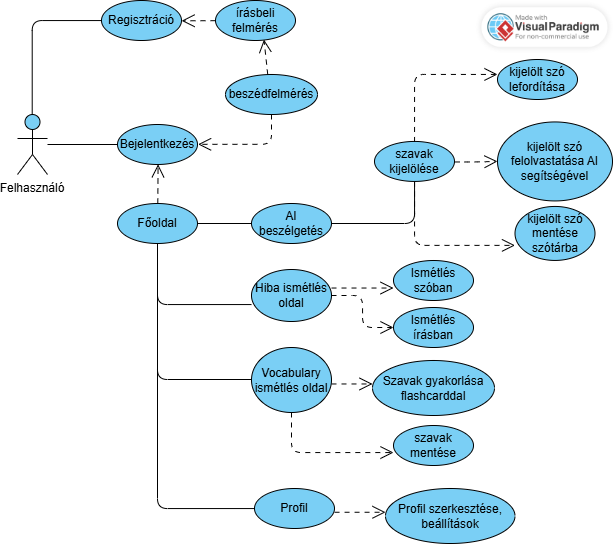
\includegraphics[width=0.9\linewidth]{images/image.png}
    \caption{Felhasználói use case diagram}
    \label{fig:usecase}
\end{figure}



\newpage

\section {Rendszerkövetelmények}

\subsection{Funkcionális követelmények}

Az alábbiakban bemutatok minden fontos funkciót az alkalmazásból.

\begin{itemize}
    \item \textbf{Regisztráció}

    A rendszer lehetőséget biztosít a felhasználó számára egy új fiók létrehozására. A regisztráció során a felhasználónak meg kell adnia a szükséges adatait. A rendszer ellenőrzni az adatokat, és hogy ki van-e töltve minden mező, formátumot ellenőriz. Ezek után ha hibát észlel a rendszer, akkor hibaüzenetet jelenít meg. A sikeres regisztráció esetén a felhasználó adatai biztonságosan eltárolásra kerülnek az adatbázisban, titkosított formában.\cite{owaspPasswordStorage}

    \item \textbf{Bejelentkezés}

    Ha már létrehozott egy fiókot a felhasználó, akkor lehetősége nyílik bejelentkezni a meglévő fiókjába. A felhasználónak meg kell adnia email címét és jelszavát. Nem megfelelő adatok esetén visszajelzést küld a hibáról a rendszer, sikeres bejelentkezés esetén pedig a rendszer hitelesítési tokent generál \cite{jwt}, amely lehetővé teszi a felhasználó számára az alkalmazás további, főbb funkcióit.

    \item \textbf{Beszélgetés a mesterséges intelligenciával}

    Az applikáción belül a felhasználóknak van lehetőségük a mesterséges intelligenciával folytatott beszélgetésre, a célnyelven. A felhasználó hang alapúan beszélgethet, vagy akár néhány mondatot írásban is küldhet a mesterséges intelligenciának. A rendszer célja, hogy a beszélgetés minél inkább hasonlítson egy valós kommunikációs helyzethez. Ennek segítségével a felhasználó tanulhatja a magabiztosabb kommunikációt.

    \item \textbf{Hibák felismerése és kezelése}

    A beszélgetés során a rendszer automatikusan felismeri a felhasználó által elkövetett nyelvi hibákat. Ezeket a hibákat kijavítja, majd eltárolja az adatbázisban, kiegészítve a helyes megoldással és szükség esetén magyarázattal. A hibák később visszakereshetők és felhasználhatók a tanulási folyamat támogatására.

    \item \textbf{Gyakorló feladatok generálása}

    A rendszer képes a felhasználó korábbi hibái alapján személyre szabott gyakorló feladatok generálására. Ezek a feladatok különböző típusúak lehetnek, például hiányos mondatok, kiejtés tanulás, szókincs alapú feladatok. A cél, hogy a felhasználó ismételten találkozzon a hibáival, és ezáltal hatékonyabban rögzítse a helyes nyelvi formákat.

    \item \textbf{Előzmények kezelése}

    A rendszer nem tárolja el a felhasználók korábbi beszélgetéseit, biztonsági okokból, viszont eltárolja a beszélgetések témájának címét, összefoglalót róla, és a hibákat, megjegyzéseket. Ennek segítségével a felhasználó nyomon tudja követni fejlődését és visszatérhet korábbi tanulási helyzetekhez.

    \item \textbf{Statisztikák}

    A rendszer különböző statisztikai adatokat gyűjt és jelenít meg a felhasználó számára, mint például a beszélgetések száma, hibák mennyisége, fejlődés üteme. Ezek az adatok segítik a felhasználót abban, hogy jobban átlássa a tanulási folyamatát.

    \item \textbf{Profil}

    A felhasználó megtekintheti és módosíthatja saját adatait a profil oldalon. Itt lehetősége nyílik a személyes beállítások, például a nyelvi szint vagy a tanulási célok módosítására.

    \item \textbf{Mesterséges intelligencia beállítások kezelése}

    A rendszer lehetőséget biztosít különböző beállítások módosítására, mint például az alkalmazás nyelve, az értesítések kezelése, az AI viselkedésének testreszabása. Ezek a beállítások hozzájárulnak a felhasználói élmény személyre szabásához.

\end{itemize}

\newpage


\newpage
\subsection{Nem funkcionális követelmények}

 Az applikáció mobil alkalmazásnak lett elkészítve, ugyanakkor a Flutter \cite{flutter} keretrendszernek köszönhetően más platformokon is használható. Gyors és stabil nyelvtanulási környezet biztosítása a cél, amely támogatja a mesterséges intelligenciával történő kommunikációt és beszédfejlesztést.

\begin{itemize}
    \item \textbf{Operációs rendszer}
    
    Az alkalmazás Android operációs rendszerre lett elkészítve, viszont más platformokon is működik. A legmegfelelőbb verziók vagy böngészők a különböző platformokon a következőek:
     \begin{itemize}
        \item \textit{Android:} 5.0 vagy újabb
        \item \textit{Web:} Google Chrome, Mozilla Firefox, Microsoft Edge aktuális verziói
     \end{itemize}
    Az alkalmazás fejlesztése során fontos szempont volt, hogy különböző képernyőméreteken és eszközökön is megfelelő felhasználói élményt nyújtson.

    \item \textbf{Tárhely}
    Az alkalmazás telepítéséhez és működéséhez legalább 250MB szabad tárhely szükséges. Később ez nőhet, eltárolt hangfájlok vagy gyorsítótározott adatok mennyiségétől függően.

    \item \textbf{Internetkapcsolat}

    Aktív internetkapcsolatra van szükség az alkalmazás működéséhez, mivel a mesterséges intelligenciával történő kommunikáció, a beszédfelismerés, valamint az adatok szinkronizálása szerveroldalon történik. Internetkapcsolat hiányában az alkalmazás bizonyos funkciói nem lesznek elérhetőek.

    \item \textbf{Teljesítmény}

    Egy nagyon fontos követelmény a gyors válaszidő. Különösen fontos szempont ez a beszélgetések során, ahol a felhasználó valós idejű kommunikációs élményt vár el. Az AI válaszgenerálásának, a beszédfeldolgozásnak és az adatbázislekérdezéseknek optimalizált módon kell működnie, azért hogy az alkalmazás folyamatos és gördülékeny felhasználói élményt biztosítson.

    \item \textbf{Megbízhatóság}

    A fejlesztés során fontos szempont volt a stabil működés és a hibák megfelelő kezelése. Különböző hibakezelési mechanizmusokat alkalmazunk annak érdekében, hogy egy esetleges hiba ne okozza az alkalmazás leállását. A backend oldalon központi hibakezelés került kialakításra, amely lehetőséget nyújt megfelelő válaszok visszaküldését a kliens számára.

    \item \textbf{Skálázhatóság}
    A rendszer úgy lett kialakítva, hogy lehetővé tehesse a további funkciók és szolgáltatások későbbi integrálását. Az AI szolgáltatások külön microszervizekként lettek elkészítve, így a rendszer könnyen bővíthetővé és fejleszthetővé vált. \cite{fowlerMicroservices} Ez lehetőség az új modellek, nyelvek, tanulási funkciók hozzáadására, anélkül hogy a teljes rendszer architektúráján módosítani kellene.

    \item \textbf{Modularitás}
    Az alkalmazás, köszönhetően a funkciók egymástól elkülönítésének, moduláris felépítést alkalmaz. Ez megkönnyíti a komponensek fejlesztését, tesztelését, cseréjét. A frontend, backend, AI szolgáltatások mind különálló részekként működnek a rendszerben.

    \item \textbf{Bővíthetőség}
    A rendszer tervezésénél a jövőre is gondoltam. Úgy lett megtervezve, hogy később új gyakorlási módokkal, új AI funkciókkal vagy további nyelvekkel bővíthető legyen. Ez a megközelítés lehetővé teszi az új módulok hozzáadását, anélkül hogy jelentős változásokat kellene végrehajtani a rendszerben.
    
\end{itemize}
